\documentclass[10pt, onecolumn]{IEEEtran}

\usepackage[utf8]{inputenc}
\usepackage{geometry}
\usepackage{listings}
\usepackage{color}
\usepackage{graphicx}
\usepackage{caption}

\geometry{margin=0.75in}

\title{Writing Assignment 2}
\author{by Mihai Dan}
\date{November 11th, 2016}


\begin{document}

    \begin{center}
        \begin{minipage}[h]{\textwidth}
            \maketitle
        \end{minipage}
    \end{center}
    
    \begin{center}
        Operating Systems II - Fall 2016
    \end{center}
    
    \newpage
    
    
    \section{Introduction}
        I/O, or input/output, is one of the fundamental needs of an operating system \cite{McGrath}. An operating system is essentially useless if it does not output results or meaningful data, which cannot be done without I/O. As with any operating system attribute, I/O is implemented in a variety of methods across different platforms. This essay will highlight the different I/O implementations used by FreeBSD and Windows, then compare them to the Linux operating system.

    
    \section{I/O Explained}
        I/O allows for external devices, such as a keyboard or monitor, to accept input from users and display appropriate output. It would be impossible for a user to communicate with an operating system without I/O functionality. There are two types of I/O, block and character. Block I/O is commonly used for memory storage systems, such as hard drives, floppy drives, and CD-ROM drives \cite{ch13}. Block I/O allows for data to move through the I/O stream in fixed-sized blocks, or chunks of data, using a large buffer for storage. On the other hand, character I/O is used when data is collected character by character and not grouped together. A simple example of a device that uses character I/O is a keyboard. As I am pressing the keys, the corresponding character is sent to the text editor, and appears on the screen as output.
        
        \vspace{1.5mm}
        
        In order for smooth I/O interaction, a system is set in place to manage these requests. This system is commonly referred to as I/O scheduling. Since each operating system has a unique way of implementing I/O scheduling, along with other I/O functionality, they will be discussed in further detail in the corresponding sections.
    
    
    \section{FreeBSD I/O and Provided Functionality}
        FreeBSD lies on the basic UNIX I/O system model, consisting of a sequence of bytes that can be accessed randomly or sequentially \cite{designO}. A typical UNIX user process has no access methods or control blocks. In most programs, the model is further simplified into the I/O stream, which is a stream of data bytes. This single common data form is what allows for the UNIX I/O model to work.
        
        \vspace{1.5mm}
        
        FreeBSD provides a plethora of data structures and algorithms regarding I/O. The most basic form of inter-process communication is the semaphore. FreeBSD handles semaphores slightly different than what we know, as they are grouped into arrays. This is done to prevent deadlock and provide better protection. Much like Linux, FreeBSD supports the implementation of queues, linked lists, and other useful data structures \cite{fkp}. One interesting feature to note is the message queue. Message queues are set up such that one process is a sender, and the other one the receiver. A lock is set in place, which a process must have in order to read or write.
        
        \subsection{Descriptors}
            Processes on FreeBSD use descriptors to reference I/O streams. Descriptors are small unsigned integers derived from the \textit{open} or \textit{socket} system calls. The \textit{open} system call creates or opens a file, specifying read and write permissions. The \textit{read} and \textit{write} system calls are used to transfer or modify data in the file. In order to de-allocate a descriptor, a call to the \textit{close} function must be made. There are three kinds of objects that can be referenced by descriptors: files, pipes, and sockets.
            
            \begin{itemize}
                \item \textit{file:} A file is a linear array of bytes that is given at least one name. A descriptor is assigned to a file by a process by calling the \textit{open} system call. A file can be removed by deleting the name and any other descriptors found in other processes.
                \item \textit{pipes:} Much like a file, a pipe is a linear array of bytes. The differences lies within the purpose of each. Pipes are unidirectional and used solely as I/O streams. A pipe is created by the \textit{pipe} system call, which consists of two descriptors; one which accepts input and one which sends it. This system also supports named pipes, or FIFOs. These named pipes exist in the filesystem, meaning they can be opened with the \textit{open} system call. Two processes communicate through a FIFO by having one open for reading and the other open for writing.
                \item \textit{sockets:} A socket is fairly different than the previously mentioned objects. A socket is solely used for inter-process communication and exists only as long as the process is alive. A socket can be created using the \textit{socket} system call, which returns its descriptor.
            \end{itemize}
            
            One important thing to note is that each process has a descriptor table, which consists of the available descriptors.
            
        
        \subsection{Devices}
            In FreeBSD, hardware devices are assigned filenames and can be accessed through the same system calls as a file. Processes do not need to make the distinction between device special file and special file, as the kernel has a function that does so. Terminals, printers, and tape drives are accessed as if they were streams of bytes, much like disk files \cite{ch13}. Most of the device dependencies and peculiarities are kept within the kernel, where they are segregated into device drivers.
            
            \vspace{1.5mm}
            
            A device driver is the entity that controls external devices and allows them to perform. Drivers in FreeBSD have three main routines.
            
            \begin{itemize}
                \item \textit{initialization:} This routine initializes the device with the appropriate software and is usually only called once.
                \item \textit{top half:} Invoked mostly from system calls and consists of routines that service I/O requests.
                \item \textit{bottom half:} Consists of the interrupt service routines.
            \end{itemize}
            
            
        \subsection{I/O Scheduling}
            FreeBSD implements the standard elevator algorithm known as C-LOOK. C-LOOK is designed to maximize throughput, but it may not always be fair to each client. This arouses the problem of starvation which is not well addressed in FreeBSD. C-LOOK is implemented using a disksort() algorithm, which sorts the requests in a cyclic, ascending order. The algorithm has a noticeable effect on the system's speed when multiple users are active. 
            
            \vspace{1.5mm}
            
            Within each device driver, there is one or more request queues. As requests arrive, they are recorded and placed into the queue. Once the action is completed, the driver receives an interrupt signal, and the request is removed from the queue. Since the I/O and interrupt service are performed in different parts of the driver, it is very important for clear communication between the top and bottom half.
    
    
    \section{Windows I/O and Provided Functionality}
        Much like any operating feature implementation, Windows has a unique way of handling I/O. The I/O system consists of several executive components that manage and provide interfaces to hardware devices. The design goal of the I/O system is to provide an abstraction of software and hardware devices to applications in the OS \cite{wio}.
        
        \vspace{1.5mm}
        
        The I/O system is dependent on the use of packets. The most common type of packet found in the Windows I/O system is the I/O request packet, or IRP. The IRP contains information relevant to the I/O request and travels between I/O system components. IRP's allow application threads to handle and serve several I/O request concurrent.
        
        \subsection{I/O System Components}
            Windows I/O system consists of several components, each with individual functionality. The components are shown in Fig. 1 and explained below.
            
            \begin{itemize}
                \item \textit{I/O manager:} The I/O manager is the heart of the I/O system. It connects applications and system components to appropriate devices.
                \item \textit{device driver:} A device driver provides the appropriate interface for a particular device. It receives commands from the I/O manager, and reports back once completed. 
                \item \textit{PnP (Plug n Play) manager:} The PnP manager guides the allocation of hardware resources amongst clients, as well as detects the removal or arrival of hardware devices.
                \item \textit{power manager:} The power manager guides the system and device drivers through power-state transitions.
                \item \textit{Windows Management Instrumentation:} The Windows Management Instrumentation allows device drivers to serve as providers.
                \item \textit{registry:} The registry is the basic database that stores the information on hardware devices.
                \item \textit{INF files:} The INF files are the driver installation files.
                \item \textit{hardware abstraction layer (HAL):} The HAL hides process specifics from the device driver through several APIs.
            \end{itemize}
		
		\begin{figure}[h]
			\centering
			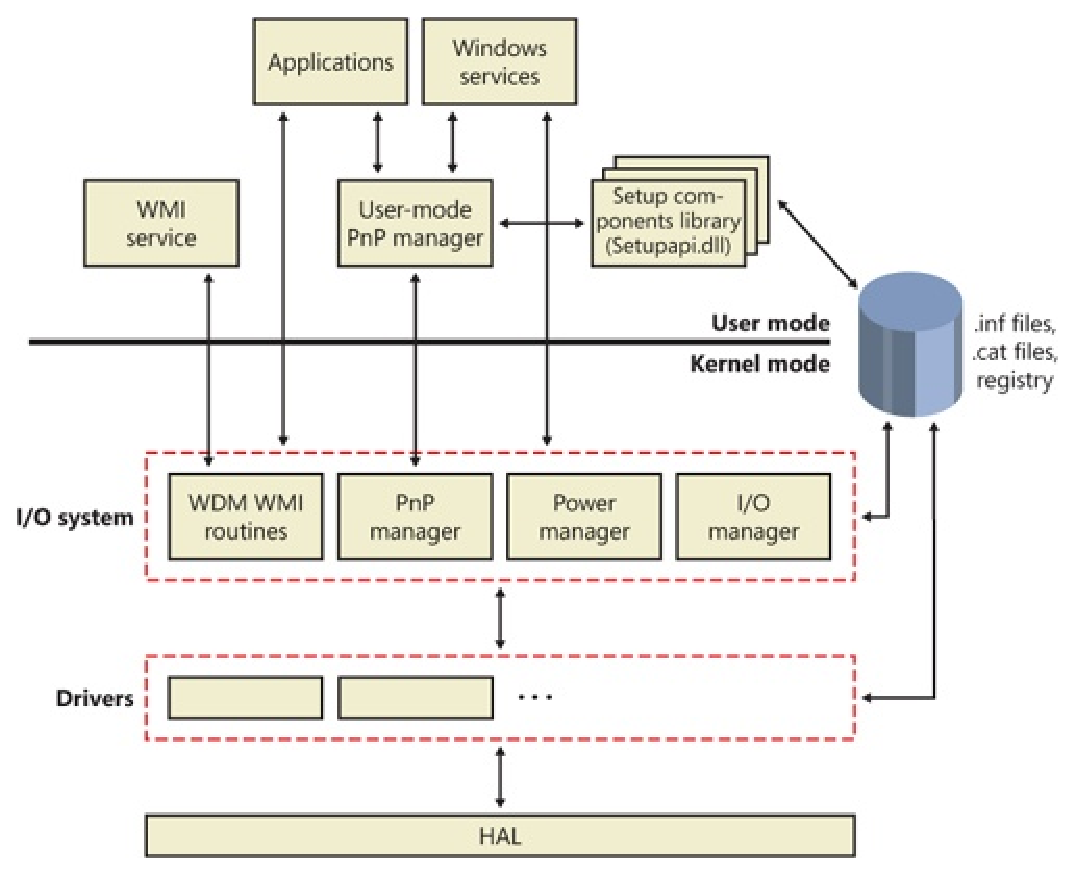
\includegraphics[width=8cm, height=5.5cm]{./pic.eps}
			\captionsetup{justification=centering}
			\caption{Visual representation of the Windows I/O System Components}
        \end{figure}
            
        \subsection{Device Drivers}
            Windows I/O System consists of two main types of drivers, file system and device drivers. File system drivers accept I/O requests from files and issues a request for the specified driver. Device drivers are used to communicate with hardware devices, such as a keyboard, mouse, or printer. There are two types of device drivers, Plug-and-Play and Non-Plug and Play \cite{wio}. Plug-and-Play drivers work with hardware devices such as mass storage devices and network adapters. These drivers consist of several steps of action in order to properly facilitate communication between devices and the system. They are as follows.
            
            \begin{enumerate}
                \item Initialization routine - performs necessary initialization
                \item Add device routine - performs necessary steps in order to add a physical device to the system, only performed with drivers that make use of PnP
                \item Dispatch routine - performs the specified action, such as read or write
                \item Start I/O routine - initiate data transfer to or from a device
                \item Interrupt service routine - signal is sent to interrupt the device
            \end{enumerate}
        
        \subsection{I/O Scheduling}
            There are a few types of I/O processing, or scheduling, available in Windows, each one designed for a specific purpose. The types of I/O processing provided by Windows are synchronous, asynchronous, Mapped File, Fast, and Scatter/Gather. Synchronous I/O is the most common type of processing. The application thread waits until the device performs the specified action and returns a status code upon completion. Once the status code is received, the program continues. An example are the \textit{ReadFile} and \textit{WriteFile}, which, in their most simple form, demonstrate synchronous I/O.
            
            \vspace{1.5mm}
            
            Asynchronous I/O allows an application to launch several I/O requests and continue executing while waiting for a response. These must be executed carefully as to avoid a thread accessing data that is being serviced by the I/O. This type improves application throughput because it allows the application to continue executing while I/O operations are in progress.
            
            \vspace{1.5mm}
            
            
            Fast I/O allows the I/O system to bypass creating an IRP and go directly to the driver stack to complete the request. This increases speed, but is not as secure. Mapped File I/O allows the OS to view a file as if it were part of the process' virtual memory. This removes the need for any disk I/O. Scatter/Gather I/O allows an application to read or write from more than one buffer in virtual memory, without needing to make several requests. As previously mentioned, each of these types are used where appropriate.
    
    
    \section{FreeBSD and Windows Compared to Linux}
        As previously mentioned, I/O is an essential need of an operating system, Linux being no exception. In this section, certain Linux I/O features will be highlighted and compared with FreeBSD and Windows.
        
        \vspace{1.5mm}
        
        One notable difference between the operating systems are the provided data structures. UNIX based operating systems, FreeBSD and Linux, rely heavily on binary trees for sorting algorithms. Windows relies on linked lists and message queues.
        
        \subsection{General I/O Management}
            As noted above, Windows uses a dedicated I/O manager and FreeBSD makes use of extensive file systems to manage descriptors. Both of these implementations differ from the Linux I/O management. Linux uses the Virtual File System (VFS), which allows for calls such as \textit{read()} or \textit{write()} to be made, regardless of file system. Another notable difference is that in Linux, the VFS and the block I/O layer are closely linked, which is not the case for Windows or FreeBSD.
        
        \subsection{Devices and Device Drivers}
            Devices are classified into three groups, block devices, character devices, and network devices. This does not differ amongst the three operating systems. One notable difference is the close connection of the block I/O and the file system. Block I/O is a lot more involved in Linux.
            
            Device drivers are also handled fairly similarly across the operating systems. A difference in the structure of the driver lies between UNIX based and non-UNIX based operating systems. Linux and FreeBSD implement a top and bottom half of the driver, while Windows does not exemplify this behavior. The initialization, execution, and clean up of these drivers is also essentially the same across these platforms.
            
        \subsection{I/O Scheduling}
            Most I/O scheduling is handled using queues, which stands true for Linux, as well as FreeBSD and Windows. In Windows, each request is represented by an IRP. Similarly, in Linux and FreeBSD, each request is represented by a request type struct. 
            
            FreeBSD uses the C-LOOK elevator scheduler, which promotes efficiency, but may not always be fair to each client. Linux has several different schedulers that may be used, but most commonly uses the Completely Fair Scheduler (CFQ). The CFQ prevents starvation by servicing the process with the least amount of CPU time. Windows makes use of several schedulers depending on the device. The most common Windows I/O scheduler is synchronous.
        
    \section{Conclusion}        
        I/O handling varies amongst different operating systems. Linux and FreeBSD tend to operate and behave similarly due to the fact that they are both UNIX based system. Windows shows the same design concepts, but has a unique way of implementation. This research shows that there is no correct way to implement I/O management; it depends on what the system is trying to accomplish.
        
    \newpage
        
    \bibliographystyle{IEEEtran}
    \bibliography{main}

\end{document}